\documentclass[border=4pt,12pt]{standalone}
% House style for redrawn exam diagrams (diagram-v4: 0.4pt lines, filled -latex arrows, fine dashes; stipple and hatching drawn as real dots/lines (no PDF/SVG patterns, so they render in every browser and at any scale); transparent background). Every figure \input's this.
\usepackage{amsmath,amssymb}
\usepackage{txfonts}
\usepackage{pdfrender,xcolor}
% \halo{text}: label on shading. The shading stops just around each letter's outline (a thin knock-out that follows the
% glyphs, like the papers' typesetting), never a box. Owner: "I don't want a box around the text".
\newcommand{\halo}[1]{\leavevmode\rlap{\pdfrender{TextRenderingMode=2,LineWidth=2.2pt,LineJoinStyle=1,StrokeColor=white,FillColor=white}#1}#1}
\usepackage{tikz,pgfplots}
\pgfplotsset{compat=1.18}
\usetikzlibrary{arrows.meta,calc,angles,quotes,patterns,patterns.meta,intersections,positioning,decorations.markings,shapes.geometric}
% Stipple and hatching are drawn as actual dots / lines clipped to the region (path picture), NOT as pattern fills:
% SVG <pattern> fills vanish or blur when browsers scale the image, so the owner could not see the shading.
% Each dot is a 0.72pt square (keeps SVGs small; reads as a dot at print size). Dots sit on one global staggered grid, so neighbouring regions line up.
\makeatletter
\newdimen\ex@x \newdimen\ex@y \newdimen\ex@xa \newdimen\ex@ya \newdimen\ex@xb \newdimen\ex@yb \newcount\ex@row
\def\exam@stipplecolor{black!75}\def\exam@dotr{0.42pt}\def\exam@dotgap{2.5}
\def\ex@rowdots{\ifdim\ex@x<\ex@xb \pgfpathrectangle{\pgfqpoint{\dimexpr\ex@x-0.36pt\relax}{\dimexpr\ex@y-0.36pt\relax}}{\pgfqpoint{0.72pt}{0.72pt}}\advance\ex@x by \exam@dotgap pt\relax\expandafter\ex@rowdots\fi}
\def\exam@stipple{%
  \pgftransformreset% dots are sized in real points even inside scaled pictures
  \pgfpointanchor{path picture bounding box}{south west}\ex@xa=\pgf@x \ex@ya=\pgf@y
  \pgfpointanchor{path picture bounding box}{north east}\ex@xb=\pgf@x \ex@yb=\pgf@y
  \pgfsetfillcolor{\exam@stipplecolor}\pgfmathsetmacro\ex@h{\exam@dotgap/2}%
  \pgfmathtruncatemacro\ex@r{floor(\ex@ya/\ex@h)-1}\ex@row=\ex@r\relax
  \ex@y=\ex@r\dimexpr\ex@h pt\relax
  \loop\ifdim\ex@y<\ex@yb
    \pgfmathtruncatemacro\ex@c{floor(\ex@xa/\exam@dotgap)-1}\ex@x=\ex@c\dimexpr\exam@dotgap pt\relax
    \ifodd\ex@row \advance\ex@x by \ex@h pt\fi
    \ex@rowdots
    \advance\ex@y by \ex@h pt \advance\ex@row by 1
    \ifnum\numexpr\ex@row-(\ex@row/4)*4\relax=0 \pgfusepath{fill}\fi% flush every 4 rows: bounded TeX memory, few clip copies in the SVG
  \repeat\pgfusepath{fill}}
\newdimen\ex@d
\def\exam@hatch#1{% #1 = 1 for /, -1 for \ ; lines 45 degrees, 3pt apart
  \pgftransformreset
  \pgfpointanchor{path picture bounding box}{south west}\ex@xa=\pgf@x \ex@ya=\pgf@y
  \pgfpointanchor{path picture bounding box}{north east}\ex@xb=\pgf@x \ex@yb=\pgf@y
  \ex@d=\dimexpr\ex@yb-\ex@ya\relax \ex@x=\dimexpr\ex@xa-\ex@d\relax
  \loop\ifdim\ex@x<\ex@xb
    \ifnum#1>0 \pgfpathmoveto{\pgfqpoint{\ex@x}{\ex@ya}}\pgfpathlineto{\pgfqpoint{\dimexpr\ex@x+\ex@d\relax}{\ex@yb}}%
    \else \pgfpathmoveto{\pgfqpoint{\ex@x}{\ex@yb}}\pgfpathlineto{\pgfqpoint{\dimexpr\ex@x+\ex@d\relax}{\ex@ya}}\fi
    \advance\ex@x by 4.24pt
  \repeat
  \pgfsetlinewidth{0.4pt}\pgfsetstrokecolor{black}\pgfusepath{stroke}}
\def\examstipple{\exam@stipple}\def\examhatch{\exam@hatch}\def\examsetstipplecolor#1{\def\exam@stipplecolor{#1}}\def\examsetdotgap#1{\def\exam@dotgap{#1}}
\makeatother
% (legacy pattern kept for old files)
% staggered stipple like the NESA papers' dotted shading
\pgfdeclarepatternformonly{exam stipple}{\pgfpointorigin}{\pgfqpoint{2.2pt}{2.2pt}}{\pgfqpoint{2.2pt}{2.2pt}}{%
  \pgfpathcircle{\pgfqpoint{0.55pt}{0.55pt}}{0.42pt}\pgfpathcircle{\pgfqpoint{1.65pt}{1.65pt}}{0.42pt}\pgfusepath{fill}}
\tikzset{
  every picture/.style={line width=0.6pt, >={Latex[length=2mm,width=1.3mm]}},
  curve/.style={line width=0.6pt},
  open arrow/.style={-{Latex[length=2mm,width=1.3mm]}},  % owner: filled -latex heads everywhere, no open chevrons
  aux/.style={dash pattern=on 2pt off 1.5pt, line width=0.6pt},
  shade/.code={\def\exA{#1}\def\exB{none}\ifx\exA\exB\else\pgfkeysalso{fill=black!18}\fi},
  shade/.default=on,
  shade dots/.style={fill=none, path picture={\examstipple}},
  stipple color/.code={\examsetstipplecolor{#1}},
  stipple gap/.code={\examsetdotgap{#1}},
  shade dense dots/.style={fill=none, stipple gap=1.6, path picture={\examstipple}},
  shade hatch/.style={fill=none, path picture={\examhatch{1}}},
  shade hatch reverse/.style={fill=none, path picture={\examhatch{-1}}},
  shade solid/.style={fill=black},
  pt/.style={circle, fill, inner sep=1.1pt},
  open pt/.style={circle, draw, fill=white, inner sep=1.1pt},
}
\pgfplotsset{
  exam axes/.style={axis lines=middle, axis line style={->}, xlabel={$x$}, ylabel={$y$},
    xlabel style={anchor=west}, ylabel style={anchor=south}, tick label style={font=\small},
    every axis plot/.append style={line width=0.6pt, black}, samples=200, clip=false,
    enlargelimits=false, axis on top},
}

\begin{document}
% coordinates in crop pixels (200 dpi), y downward; curve traced from the crop (sketch, flatter tails than a true normal)
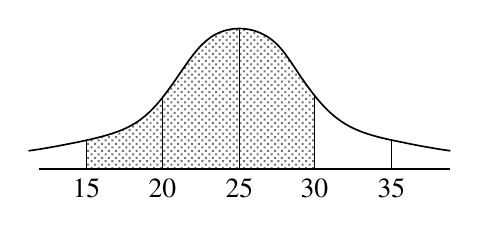
\begin{tikzpicture}[x=0.0127cm, y=-0.0127cm, every node/.style={font=\normalsize}]
  \fill[shade dots, stipple color=black!55] (64,146) -- plot[smooth] coordinates {(64,117.2) (69.46,116.1) (74.93,114.9) (80.24,113.5) (85.51,111.9) (90.67,110.2) (95.68,108.3) (100.6,106.2) (105.4,103.9) (110.1,101.5) (114.6,98.83) (118.8,96.01) (123,92.97) (126.9,89.71) (130.7,86.24) (134.4,82.48) (138,78.54) (141.4,74.39) (144.7,70.1) (148,65.57) (151.1,60.95) (154.2,56.18) (157.3,51.18) (160.4,46.03) (163.5,41.03) (166.5,36.35) (169.6,31.9) (172.7,27.86) (175.9,24.19) (179.2,20.94) (182.7,18.02) (186.5,15.34) (190.5,12.97) (194.6,10.93) (199,9.216) (203.4,7.846) (207.9,6.83) (212.5,6.179) (217.1,5.903) (221.6,6.008) (226.1,6.497) (230.5,7.38) (234.7,8.643) (238.7,10.3) (242.6,12.34) (246.5,14.8) (250.4,17.67) (254.1,20.84) (257.6,24.31) (261.1,28.11) (264.3,32.08) (267.4,36.3) (270.5,40.85) (273.5,45.59) (276.6,50.62) (279.6,55.72) (282.7,60.57) (285.7,65.17) (288.8,69.49) (292,73.5)} -- (292,146) -- cycle;
  \draw[curve] plot[smooth] coordinates {(6,128) (16.2,126.5) (26.27,124.8) (36.33,123) (46.6,121) (56.72,119) (66.91,116.8) (76.41,114.5) (85.45,112) (93.79,109.3) (101.6,106.2) (108.8,102.6) (115.4,98.64) (121.4,94.11) (127.5,88.73) (133.3,82.69) (139.1,75.92) (144.7,68.6) (150.6,60.48) (156.5,51.87) (162.4,43.35) (168.1,35.38) (173.7,28.33) (179,22.35) (184.4,17.42) (189.8,13.45) (195.3,10.43) (201.3,8.085) (207.5,6.535) (214,5.752) (220.5,5.796) (227,6.675) (233.4,8.351) (239.4,10.77) (245.2,13.96) (250.5,17.82) (255.6,22.52) (260.7,28.34) (265.9,35.34) (271.5,43.53) (277.3,52.23) (283.1,60.61) (288.8,68.38) (294.5,75.65) (300.4,82.36) (306.4,88.47) (312.5,93.84) (319,98.62) (325.6,102.7) (332.6,106.2) (340.3,109.4) (348.6,112.1) (357.6,114.6) (367,116.8) (377.1,118.9) (387.4,121) (397.7,123) (407.8,124.8) (417.8,126.5) (428,128)};
  \draw (17,146) -- (428,146);
  \draw (64,146) -- (64,117.2);
  \node[below] at (64,146) {$15$};
  \draw (140,146) -- (140,76.0);
  \node[below] at (140,146) {$20$};
  \draw (217,146) -- (217,6.0);
  \node[below] at (217,146) {$25$};
  \draw (292,146) -- (292,73.5);
  \node[below] at (292,146) {$30$};
  \draw (369,146) -- (369,117.0);
  \node[below] at (369,146) {$35$};
\end{tikzpicture}
\end{document}
